\chapter{Analyse}
%Evaluation der SAP Business Technology Platform für die Anforderungen auf dem deutschen Kfz-Versicherungsmarkt
\section{Task Charakteristika - Anforderungen der Kfz-Versicherer an digitale Plattformen}

\subsection{Literaturbetrachtung aktueller Anforderungen an digitale Plattformen}

\improvement{Optimierung der Quellen bei den Anforderungen}

Im Nachfolgenden werden die in der Literatur gefundenen Anforderungen unter den Punkten 1-16 beschrieben. Eine Übersicht über die identifizierten Anforderungen ist in Abbildung ... dargestellt.

\begin{figure}[h]
    \centering
    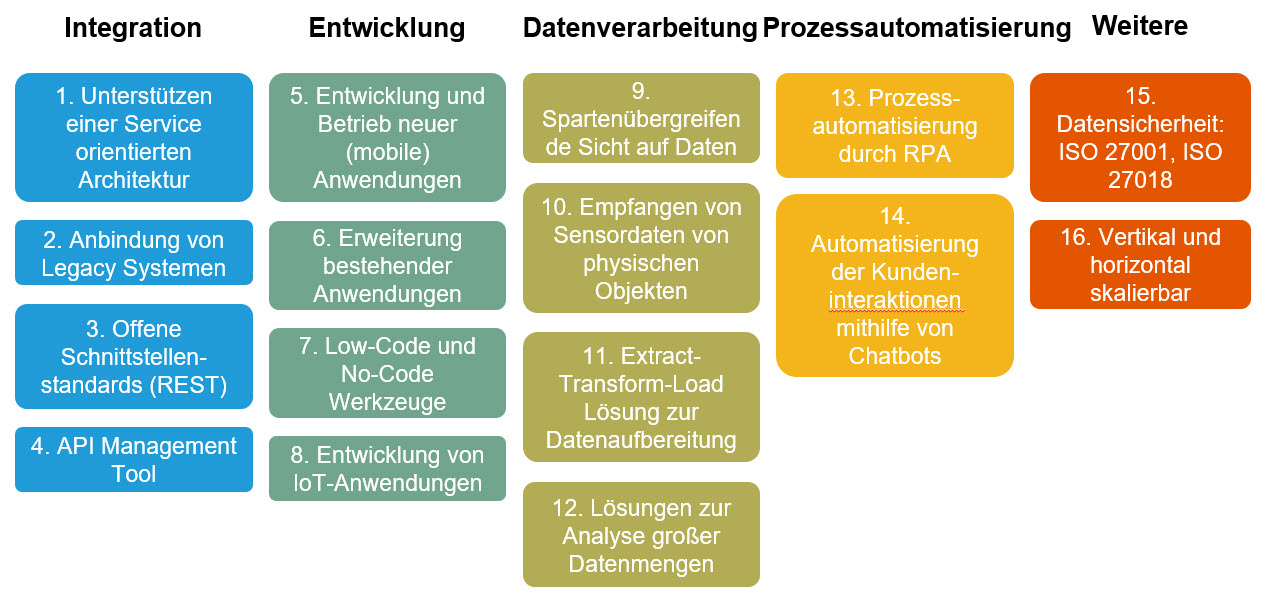
\includegraphics[width=1\textwidth]{img/PP_Anforderungen.jpg}
    \caption[Anforderungen der Kfz-Versicherer an digitale Plattformen]{Anforderungen der Kfz-Versicherer an digitale Plattformen\autocite{PPAnf}}
    \label{fig:PPAnf}
\end{figure}
\footnotetext{eigene Darstellung}

Eine der größten Herausforderungen, denen sich Kfz-Versicherungsunternehmen stellen müssen, sind die historisch bedingten IT-Landschaften, die auch als IT-Legacy oder Legacy-Systeme bezeichnet werden. Diese führen aufgrund der starken Abhängigkeit zwischen den einzelnen Systemen sowie der monolithischen Programmstruktur häufig zu langen Entwicklungszyklen. \autocite[Vgl.][S. 10-12]{GUNTER2020}

%Diese sind seit Beginn der 1970er Jahre entstanden und wurden dabei größtenteils von den Versicherern selbst entwickelt. Mittlerweile führt allerdings genau diese IT-Legacy aufgrund der starken Abhängigkeiten zwischen den Systemen und der monolithischen Programmstruktur häufig zu langen Entwicklungszyklen (vgl. S. 10-12 Gunter2020) 

(1) Um dennoch schnell auf die sich ändernden Kundenbedürfnisse und Marktbedingungen reagieren zu können, muss eine technologische Plattform für Kfz-Versicherer eine \textbf{Service-orientierte Architektur (SOA) unterstützen}. Dabei erleichtert der modulare Aufbau einer SOA das Hinzufügen und Entfernen von neuen Anwendungen an der Kundenschnittstelle \autocite[Vgl.][S. 392]{WARG2016} und ermöglicht es, abgeschlossene Programmelemente wie beispielsweise die Rechenkerne der verschiedenen Versicherungssparten als gekapselter Service in eine neue IT-Landschaft einzubinden \autocite[Vgl.][S. 10f]{URLA2019}

(2) Weiterhin befinden sich in den Legacy-Systemen der Versicherer sehr viele wichtige Daten, welche für die Tarifierung benötigt werden und teilweise aus regulatorischen Gründen noch aufbewahrt werden müssen. Daher müssen die bestehenden Legacy-Systeme der Versicherer an die technische Plattform angebunden oder die Daten in neue Systeme migriert werden. Da letzteres sehr kosten- und zeitaufwändig ist, muss eine digitale Plattform für Kfz-Versicherer \textbf{die Anbindung der Legacy-Systeme} ermöglichen. \autocite[Vgl.][S. 10-12]{GUNTER2020}

(3) Ein Trend, der insbesondere in den nächsten Jahren die Versicherungsbranche bestimmen wird, sind die sogenannten digitalen Ökosysteme und die damit verbundenen Partnerschaften \autocite[Vgl.][]{AVRAMAKIS2023}.  So erachten gemäß einer Studie der Swiss RE aus dem Jahr 2019 mehr als 75\% der Führungskräfte von Versicherungsunternehmen weltweit digitale Ökosysteme und andere Partnerschaften als wesentlich für die Schaffung von Wettbewerbsvorteilen. \autocite[Vgl.][]{PAYNE2022} Für die Partizipation an digitalen Ökosystemen ist dabei vor allem das Vorhandensein offener Standardschnittstellen und Austauschformate maßgebend, sodass ähnlich wie im Banking mit der PDS2 Richtlinie auch Versicherungsunternehmen ihre Daten leicht mit Partnern und Drittanbietern teilen können. Zu diesem Zweck hat sich 2018 \autocite[Vgl.][]{2021z} die Free Insurance Data Initiative (FRIDA) gebildet, welche für die einzelnen Versicherungssparten branchenweite API-Standards etablieren möchte. Im Kfz-Bereich stellt FRIDA die Car-Claims API bereit, welche als REST-API den Austausch von Kfz-Police-Daten vereinfachen soll. Folglich sollte eine Plattform für Kfz-Versicherer \textbf{Standard-API-Formate} wie REST \textbf{unterstützen}, um sich mit Partnern und InsurTechs in einem digitalen Ökosystem verbinden zu können und somit wettbewerbsfähig zu bleiben. \autocite[Vgl.][]{KRETZ2023}

(4) Zudem sollte die Plattform über ein \textbf{API-Management-Tool} verfügen, sodass Kfz-Versicherer bei der Vielzahl an Schnittstellen nicht die Übersicht verlieren und API-Aufrufe sowohl im als auch außerhalb des Unternehmens analysiert, kontrolliert und verwaltet werden können. \autocite[Vgl.][S. 67ff]{HANSCHKE2021}

(5) Neben der Entwicklung und dem Betrieb von klassischen Webanwendungen muss die Plattform auch \textbf{mobile Applikationen} unterstützen, da immer mehr Kunden ihre Mobilgeräte nutzen, um auf Versicherungsdienstleistungen zuzugreifen und diese zu verwalten. So können Mobile Apps beispielsweise bei einem Autounfall dazu verwendet werden, den eigenen Standort sowie Fotos vom Schaden zu teilen. \autocite[Vgl.][S. 7]{HU2020}

(6) Darüber hinaus sollte es die Plattform ermöglichen, \textbf{bestehende Anwendungen} mithilfe von kleinen Programmcodes \textbf{eigenständig erweitern} zu können, um die Anwendungen nach den Bedürfnissen der Kfz-Versicherer anpassen zu können. \autocite[Vgl.][]{WEINGARTNER2023}

(7) Hierbei gilt es zu berücksichtigen, dass insbesondere bei kleinen und mittelgroßen Versicherern die Entwicklungsressourcen sehr knapp sind. Daher sollte die Plattform ebenfalls sogenannte \textbf{Low- oder besser No-Code-Werkzeuge bereitstellen}, damit auch Nutzer aus den Fachabteilungen kleine Applikationen sowie Erweiterungen erstellen können.(vgl. VBLOWCODE2022) \autocite[Vgl.][]{VBLOWCODE2022}

(8, 9) Ein weiterer Trend, der die letzten Jahre insbesondere bei jungen Fahrern sehr beliebt ist, sind Telematik-Tarife. Telematik bezeichnet dabei allgemein die Verbindung von Informatik und Telekommunikation, \autocite[Vgl.][S. 10-11]{ABTS2017} und ermöglicht in der Kfz-Versicherungsbranche die Berücksichtigung des individuellen Fahrverhaltens des Versicherungsnehmers sowie anderer externer Rahmenbedingungen bei der Prämienbestimmung \autocite[Vgl.][S. 84]{MERZINGER2017}. So kann der Versicherer seine Produkte besser an das Risikoprofil seiner Kunden anpassen und die Kunden bei einer zurückhaltenden Fahrweise von günstigeren Preisen profitieren. Hierfür werden mithilfe von Sensoren im Auto verschiedene Daten zum Fahrstil des Nutzers erfasst und zur Tarifierung an den Versicherer übermittelt. \autocite[Vgl.][S. 3-4]{ELING2020} Für den Einsatz von technologischen Plattformen bei Kfz-Versicherern ist es folglich wichtig, dass die Plattform \textbf{Sensordaten von physischen Objekten in Echtzeit empfangen kann} \autocite[Vgl.][S. 10-15]{WEICHERT2015}. Zudem sollte die Plattform auch Möglichkeiten zur \textbf{Entwicklung von IoT-Anwendungen} bereitstellen, um Sensordaten in Geschäftsprozesse integrieren zu können. 

(10) Die zu Anfang erwähnte Herausforderung der Altsysteme zeigt sich auch in der Datenverarbeitung. So verhindern die fragmentierten IT-Landschaften der Versicherer eine integrierte Sicht auf die Daten, sodass eine \textbf{spartenübergreifende Betrachtung} aktuell nicht möglich ist. \autocite[Vgl.][S. 11]{GUNTER2020}

(11) Ergänzend ist im Rahmen des Datenmanagements wichtig, sicherzustellen, dass die Daten in einem konsistenten und strukturierten Format vorliegen, sodass auf dieser Grundlage eine effektive Analyse und Verwaltung der Daten möglich ist. Folglich muss die Plattform eine \textbf{Extract-Transform-Load-Lösung ((\acs{etl})-Lösung)} bereitstellen, um Daten aus verschiedenen Quellen zu extrahieren, sie zu transformieren und schließlich in ein Zielsystem zur Analyse laden zu können. \autocite[Vgl.][]{WEINGARTNER2023}

(12) Durch die Technologisierung der Automobilbranche und der umfassenden Datenerhebung im Fahrzeug, hat sich die Kfz-Versicherung als Vorreiter der Assekuranz im Bereich Data Analytics hervorgetan. \autocite[Vgl.][S. 187]{GATZERT2023} Die Auswertung der großen Datenmengen ermöglicht eine genauere Abschätzung bestehender Risiken und führt somit zu einer exakteren Kalkulation von Prämien. Dies ist auf die Anwendung der Wahrscheinlichkeitstheorie zur Prämienberechnung zurückzuführen, bei der ein höheres Ausmaß an untersuchten Fällen zu einem präziseren Ergebnis führt. Folglich sollte eine technologische Plattform für Kfz-Versicherungen \textbf{Lösungen zur Analyse großer Datenmengen} zur Verfügung stellen, um den Kfz-Versicherern eine optimale Tarifierung zu ermöglichen \autocite[Vgl.][S. 146]{MANGEI2019}. 

(13) Neben den bestehenden Legacy-Systemen und der Wertschöpfung aus Daten, haben zahlreiche Kfz-Versicherer mit internen repetitiven Prozesse zu kämpfen, die manuell von Mitarbeitern ausgeführt werden müssen. Dies führt zu langen Bearbeitungszeiten, Anfälligkeit für menschliche Fehler und einer Bindung von wertvollem Humankapital, das nicht für die Kundenbetreuung eingesetzt werden kann. Eine Lösung zur Bewältigung dieser Herausforderung, die auch von der technologischen Plattform unterstützt werden sollte, ist die \textbf{Robotic Process Automation} (RPA). So können repetitive Aufgaben wie beispielsweise die Übertragung von Daten in Systeme, das Erstellen von Berichten oder das Überprüfen von Schäden automatisiert werden. \autocite[Vgl.][S. 296-298]{REICH2019}  Die Allianz vermutet, dass durch den Einsatz von RPA die Arbeitszeit um 40\% reduziert und gleichzeitig die Qualität der Leistung verbessert werden. Dies betont noch einmal die Bedeutung von RPA für die Wettbewerbsfähigkeit in der Branche. \autocite[Vgl.][S. 296-298]{REICH2019}

(14) Gemäß Reich (2019) besteht eine zusätzliche Option für die Automatisierung von Kundeninteraktion in der Kfz-Versicherungsbranche bei Fällen wie Anträgen, Auskünften oder Schadensmeldungen durch den Einsatz von Chatbots. So können Fragen von Kunden, insbesondere solche, die sich auf Versicherungspolicen, Abrechnungen oder Schadensmeldungen beziehen, jederzeit beantwortet werden, ohne dass der Kunde auf einen Mitarbeiter warten muss. Dadurch kann der Bedarf nach Mitarbeitern in der Sachbearbeitung reduziert und die Kundenzufriedenheit erhöht werden, weshalb die Plattform für Versicherer auch \textbf{Chatbot-Funktionalitäten} bereitstellen sollte. \autocite[Vgl.][S. 300-302]{REICH2019}

(15) Die strikten regulatorischen Anforderungen innerhalb der Versicherungsbranche erfordern eine ausgeprägte \textbf{Datensicherheit} für alle verwendeten Softwarelösungen, einschließlich technischer Plattformen. Da die individuelle Überprüfung des Sicherheitsniveaus zu aufwändig ist, greifen Versicherungsunternehmen in der Praxis auf Zertifizierungen und Testate zurück. \autocite[Vgl.][S. 777]{ZDANOWIECKI2016} Die ISO/EIC 27001 Norm dient dabei als Standard für Cloud-basierte Lösungen. Zusätzlich müssen Kfz-Versicherer sicherstellen, dass die Verarbeitung von personenbezogenen Daten den Vorschriften der Datenschutzgrundverordnung (DSGVO) entspricht. Hierfür wurde der Standard ISO/EIC 27018 festgelegt. Folglich sollte eine technische Plattform für Kfz-Versicherer sowohl \textbf{nach ISO/EIC 27001 als auch nach ISO/EIC 27018 zertifiziert} sein. 
\improvement{Fehlt hier ein Zitat}

(16) Eine weitere Anforderung, die ebenfalls von Beginn an erfüllt sein sollte, ist die Fähigkeit der \textbf{Plattform zur horizontalen und vertikalen Skalierbarkeit}. Dies erfordert, dass die Plattform zusätzliche Server automatisch starten und Lasten auf mehrere Server verteilen kann, um hohe Nutzerzahlen zu bewältigen, wie sie speziell im Herbst bei Kfz-Versicherern aufgrund des verstärkten Wechsels von Versicherungsnehmnern vorkommen können. (horizontale Skalierbarkeit). Des Weiteren muss die Plattform in der Lage sein, je nach Bedarf die Rechenleistung und Speicherkapazität des Servers zu erhöhen, um einem höheren Ressourcenbedarf gerecht zu werden (vertikale Skalierbarkeit). \autocite[Vgl.][S. 23]{JAHNERT2020}

\subsection{Evaluation und Ergänzung der Anforderungen aus Sicht der Experten}

\improvement{Hier die Punkte der Bafin noch mit dazunehmen}

\improvement{Umformulieren der Anforderung API-Tool zu offene Schnittstellenstandards wie im Interview}

Die zuvor aus der Literatur herausgearbeiteten Anforderungen konnten von allen Experten bestätigt werden. Hervorgehoben wurde dabei insbesondere, dass der Preis für den Endkunden der alles entscheidende Faktor ist und daher aktuell alle Kfz-Versicherer versuchen, ihre komplette Lieferkette zu digitalisieren. Dabei wurde ebenfalls die Unterstützung von mobilen Anwendungen als sehr wichtig betont, um dort dann beispielsweise Tätigkeiten wie das Buchen eines Werkstatttermins durchzuführen. 

Des Weiteren wurde von Experte 1 das Unterstützen einer „Entkopplungsarchitektur“ als Anforderung genannt, damit Kfz-Versicherer agil an der Kundenschnittstelle agieren und gleichzeitig auf die statischen Informationen aus den Altsystemen zugreifen können.\autocite[Vgl.][]{LEMONIDIS2023} Die dafür notwendige Kapselung der Altsysteme und das Bereitstellen dieser über Schnittstellen unterstützt im Wesentlichen die Anforderung einer SOA. Zudem wurde von Experte 2 die leichte Integration der Kfz-Versicherer in Ökosysteme und Vertriebskanäle wie Check24 mit den Schlagworten Open Insurance und Embedded Insurance betont.\autocite[Vgl.][]{GREBERT2023} Beide werden im Rahmen dieser Arbeit unter der Anforderung offene Schnittstellenstandards zusammengefasst, da diese die dafür notwendige Voraussetzung sind. Weitere Anforderungen, die von den Experten ergänzt wurden, werden im Folgenden kurz vorgestellt.

(17) Entscheidungsfindung durch KI – Für Experte 2 stellte zudem das Unterstützen der Kfz-Versicherer bei der Entscheidungsfindung durch KI Modelle in Prozesse wie der Akquise oder dem Schadensprozess eine weitere Anforderung dar, um bestimmte Sachverhalte prüfen zu lassen.\autocite[Vgl.][]{GREBERT2023} 

(18) Bereitstellung einer Prozessorchestrierungslösung – Aus Sicht des Experten 3 ist es für Kfz-Versicherer zudem wichtig, dass die Plattform ein Prozessorchestrierungstool bereitstellt, mit dem Prozesse systemübergreifend end-to-end designt, verwaltet und gezielt Prozessschritte in den jeweiligen Lösungen über Schnittstellen angesteuert werden können. \autocite[Vgl.][]{SCHMIDT2023} 

(19) Wenig Wartungsaufwand – Für Experte 3 stellte eine weitere grundlegende Anforderung die einfache Wartbarkeit der Plattform dar, sodass beispielsweise neue Releases automatisch eingespielt und damit die neuesten Technologien direkt bereitgestellt werden können. \autocite[Vgl.][]{SCHMIDT2023} 

(20) Contentpakete – Aus Sicht des Experten 3 sollte eine technische Plattform neben den bereitgestellten Tools in den einzelnen Clustern auch Contentpakete bereitstellen. Mit dem Begriff Content sind dabei Inhalte gemeint, die den Implementierungsaufwand in den einzelnen Bereichen reduzieren. Das können bspw. vordefinierte Schnittstellen, Adaptoren oder auch vordefinierte Frameworks sein. \autocite[Vgl.][]{SCHMIDT2023} 

\begin{figure}[h]
    \centering
    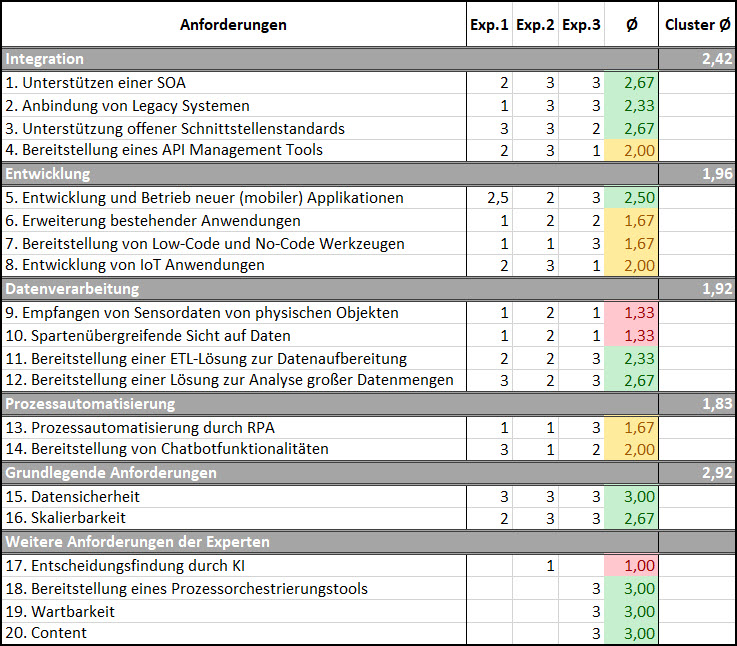
\includegraphics[width=1\textwidth]{img/Gewichtung_Anforderung.jpg}
    \caption[Gewichtung der Anforderungen durch die Experten]{Gewichtung der Anforderungen durch die Experten\autocite{Gewichtung}}
    \label{fig:Gewichtung}
\end{figure}
\footnotetext{eigene Darstellung}
\improvement{Aufpassen wo Tabelle hinrutscht}

Nach Überprüfung und Ergänzung der in der Literatur gefundenen Anforderungen, wurden die Anforderungen von den Experten ebenfalls nach ihrer Wichtigkeit in den nächsten 3-5 Jahren priorisiert. Die Aufgaben wurden nach Themen gruppiert und die Bewertung durch die Experten zunächst einzeln aufgeführt und dann Durchschnittswerte je Anforderung und je Cluster gebildet. Die Experten konnten einen Wert von 1-3 vergeben, wobei 1 für eine niedrige, 2 für eine mittlere und 3 für eine hohe Priorität steht. Wurden von einem Experten weitere Anforderungen benannt und diese im Rahmen der Analyse zu bereits identifizierten Anforderungen dazugezählt, wird für die Priorisierung der Anforderung der Mittelwert gebildet.

\improvement{Zahlen ausschreiben}

\improvement{Positionierung der Tabelle}

Anhand der Tabelle ist zu erkennen, dass die Experten die einzelnen Anforderungen zwar teilweise sehr unterschiedlich bewerten, sich aber dennoch einige Tendenzen erkennen lassen. So sind neben den grundlegenden Erfordernissen Datensicherheit und Skalierbarkeit insbesondere die Anforderungen im Bereich der Integration besonders wichtig. 

%Darauf folgend sind mit einem Durchschnittswert von ca. 1,9 die weiteren Anforderungsgruppen für in etwa gleich wichtig befunden worden. 









\section{Technologie Charakteristika - Komponenten und Services der SAP Business Technology Platform}\label{sec:TechCharak}

\improvement{BTP Punkte runder und knapper formulieren, hier könnten die Punkte die früher in Word in 2.1.4 standen, helfen}
\improvement{Überschrift kürzer}

Aufgrund des umfangreichen Serviceportfolios der SAP BTP sowie des begrenzten Umfangs dieser Arbeit werden im Folgenden nur die Kernfunktionalitäten der BTP in den Bereichen Datenmanagement, Datenanalyse, Anwendungsentwicklung, Integration und intelligente Technologien vorgestellt. Grundsätzlich lässt sich festhalten, dass die Services der einzelnen Bereiche als Cloud Service konsumierbar sind und daher Cloud-Eigenschaften wie Elastizität, Skalierung und Hochverfügbarkeit erfüllen. \autocite[Vgl.][S. 60]{SEUBERT} Zudem ist die SAP BTP nach den Standards ISO27001, ISO27017, ISO27018, ISO22301 und C5(ISAE3402) zertifiziert und entspricht damit den gängigen Anforderungen an die Datensicherheit.(vgl. \ref{sec:BTPZertifikate}) Die Services aus den einzelnen Bereichen bauen dabei auf den sogenannten Foundational Services auf. Diese umfassen beispielsweise ein Identity Service zur Authentifizierung, ein Audit-Log-Service zum Aufzeichnen von sicherheitsrelevanten Handlungen oder einen Application Autoscaler Service zur automatischen Skalierung von Anwendungen. \autocite[Vgl.][S. 58]{SEUBERT}

\improvement{Abbildung als Übersicht über die BTP einbauen}

Im Bereich des \textbf{Datenmanagements} lassen sich mit der SAP BTP verschiedene Datenarchitekturen wie beispielsweise eine zentrale Datenplattform oder ein Data Fabric realisieren. Diese können aufgrund des Plattformansatzes kontinuierlich weiterentwickelt und miteinander kombiniert werden. Für die transaktionale Verarbeitung von Daten kann der Datenbankservice SAP HANA Cloud der BTP verwendet werden, um Daten gemäß ihrer Eigenschaften zu organisieren und zu verarbeiten. Darüber hinaus ermöglicht der Data Intelligence Service der BTP den Aufbau einer Data Fabric Architektur. \autocite[Vgl.][S. 64-66]{SEUBERT} So können mit dem Service unstrukturierte und strukturierte Daten aus verschiedenen Quellen ( Datenbanken, IT-Anwendungen, Dateisysteme, Cloud-Service) unabhängig vom Betriebsmodell der Datenquelle integriert werden. Zudem können, die für die Integration und Verarbeitung der Daten erforderlichen Aufgaben vom Data Intelligence Service orchestriert werden. \autocite[Vgl.][]{DATAINTELLIGENCE} Zur Aufbereitung der Daten kann der SAP Datasphere Service eingesetzt werden. Dieser kann die Daten aus den unterschiedlichen Systemen föderieren, transformieren und zur Auswertung in ein dafür geeignetes Zielsystem, wie die SAP Analytics Cloud laden. \autocite[Vgl.][S. 3]{FSDDATASPHERE}  Dabei gilt es zu erwähnen, dass der Datasphere Service langfristig die Integrationsfunktionalitäten des Data Intelligence Services übernehmen soll. \autocite[Vgl.][]{QUIRK2023}

Die Funktionalitäten und Services der SAP BTP zur \textbf{Datenanalyse} bauen auf den Services des Datenmanagements auf, da die Daten für die Analyse in einer strukturierten Form bereitgestellt werden müssen. Der zentrale Service wird dabei von der SAP Analytics Cloud repräsentiert, welche als \ac{saas}-Produkt Funktionen für Business Intelligence, Unternehmensplanung und die prädiktive Analysen zur Verfügung stellt. Mit den Selfservice-Funktionen für BI können die aufbereiteten Daten von Graphen, Tabellen und Karten in einem einheitlichen Dashboard visualisiert und als Bericht geteilt werden. Darüber hinaus ermöglicht die SAC Business Reporting, indem die Nutzer durch verschiedene Filter- und Drill-Down-Funktionen mit den Darstellungen interagieren und Zusammenhänge aufdecken können. Für die Unternehmensplanung können mit der SAC Finanz- und Betriebspläne in Form von Tabellen erstellt und miteinander verknüpft werden, um Auswirkungen von veränderten Planungseingaben auf andere Unternehmensbereiche direkt zu erkennen. Mithilfe prädiktiver Analysen können zudem auf der Grundlage historischer Daten Prognosen erstellt werden, die direkt in die Einsatzplanung integriert werden können. \autocite[Vgl.][S. 64-67]{SEUBERT} Dazu können die ausgewählten Datensätze mithilfe von Klassifikations-, Regressions- und Zeitreihenanalysen untersucht werden. \autocite[Vgl.][]{FSDSAC2023}

Neben dem Datenmanagement und der Datenanalyse stellt die SAP BTP ebenfalls Funktionalitäten für die \textbf{Anwendungsentwicklung} bereit, welche verschiedenen Abschnitte des Softwarelebenszykluses adressieren. Abhängig von den jeweiligen funktionalen Anforderungen können die Anwendungen bzw. Erweiterung auf unterschiedlichen Laufzeitumgebungen entwickelt werden. Hierzu gehören die Cloud Foundry Runtime Environment zur Entwicklung von Microservices basierenden Erweiterungen, das SAP BTP ABAP Environment zur Entwicklung und Bereitstellung von ABAP Anwendungen, sowie SAP Kyma für containerbasierte Anwendungen und Erweiterungen. Zudem stellt die BTP zur Vereinfachung der Entwicklung mit dem Business Application Studio eine IDE und mit dem Cloud Application Programming (CAP) ein Framework für die Programmiersprachen Java und Node.js bereit \autocite[Vgl.][S. 67-69]{SEUBERT} Zusätzlich werden von der SAP BTP mit dem sogenannten Mobile Service ebenfalls die Entwicklung von nativen und plattformübergreifenden mobilen Apps unterstützt. \autocite[Vgl.][S. 217-219]{SEUBERT} Neben diesen Tools für die professionelle Entwicklung ermöglicht die BTP mit dem SAP Build Apps Service auch Citizen Developern die Realisierung und Erweiterung von Geschäftsanwendungen. So stellt der Service Low-Code und No-Code Tools bereit mit den Business-User bestehende Anwendungen im Drag-and-Drop Verfahren erweitern sowie neue Anwendungen bauen können. \autocite[Vgl.][S. 4]{SAPBUILDAPPS}

\improvement{die Funktionen der Anwendungsentwicklung werden auch als Extension Suite bezeichnet --> wichtig für Gartner}

Die \textbf{Integrationsservices} der SAP BTP werden im Wesentlichen durch die Integration Suite repräsentiert, welche mehrere Services zur Integration umfasst. Einer davon ist der Connectivity Service mit dem On-Premise Systeme an die SAP BTP über Cloud-Konnektoren angebunden werden können. \autocite[Vgl.][]{CLOUDCONNECTOR} Diese Cloud-Konnektoren unterstützen HTTP und \ac{rfc}-Protokolle für die Kommunikation und haben gegenüber herkömmlichen Ansätzen den Vorteil, dass keine Änderung der Firewall-Konfiguration notwendig ist. Mit dem Service SAP Open Connectors wird darüber hinaus die Integration von über 150 Nicht-SAP-Cloud Anwendungen, wie z.B. Microsoft Dynamics, Salesforce oder Sage mithilfe von vorkonfigurierten Konnektoren vereinfacht. \autocite[Vgl.][S. 28]{INTEGRATIONSUITE2023} Neben der Integration von Anwendungen und Prozessen über Protokolle und dazugehörige Adapter, unterstützt die BTP ebenfalls Events sowie REST, SOAP und ODATA APIs für die Anbindung von Anwendungen. \autocite[Vgl.][]{BTPAPIS2023} Die eventbasierte Kommunikation erfolgt hierbei über den SAP Event Mesh Service.  \autocite[Vgl.][S. 4]{EVENTMESH2022} Weitere wichtige Services im Bereich der Integration sind die Iot Services der BTP, welche unter dem Begriff SAP Internet of Things zusammengefasst werden. \autocite[Vgl.][S. 163]{SEUBERT} Die IoT Services ermöglichen die Kommunikation mit physischen Geräten, sowie die Speicherung und Analyse von Sensordaten. So können Daten von physischen Objekten wie beispielsweise eines Autos Maschine direkt in Geschäftsprozesse integriert werden. \autocite[Vgl.][]{IOTBTP2023}  Zur Verwaltung und Kontrolle der unterschiedlichen Schnittstellen kann der API Management Service der BTP eingesetzt werden. \autocite[Vgl.][S. 72]{SEUBERT} 

Um Abläufe und Prozesse im Unternehmen zu optimieren und intelligenter umzusetzen, stellt die SAP BTP mehrere Services im Bereich \textbf{intelligente Technologien} bereit, die auf künstlicher Intelligenz und ML aufbauen.  Ein zentraler Service ist hier SAP Build Process Automation, welcher sich aus den Teilbereichen Workflow Management und Robotic Process Automation zusammensetzt. Für die Automatisierung von Prozessen können mit dem Service sowohl beaufsichtige als auch unbeaufsichtigte Bots entwickelt werden. Hierfür werden die zu automatisierenden Aktivitäten eines menschlichen Users in einer Benutzeroberfläche aufgezeichnet, sodass diese Interaktionen nachfolgend vom Bot emuliert werden können. Neben der Entwicklung von Bots werden über die BTP bereits mehr als 180 vordefinierte Bots für ausgewählte Anwendungsszenarien zur Verfügung gestellt. \autocite[Vgl.][S. 74-76]{SEUBERT} Zusätzlich lassen sich über den Workflow Editor end-to-end Prozesse mittels Drag and Drop Funktionalitäten erstellen und erweitern. Über die Funktion Process Visibility des Services können die Prozesse und Automatisierungen über ein Dashboard verwaltet und überwacht werden. Dadurch lassen sich beispielsweise Engpässe bei der Prozessbearbeitung erkennen und unterschiedliche Kennzahlen wie die Anzahl offener oder abgeschlossener Prozessabläufe einsehen. \autocite[Vgl.][S. 5]{FSDBPA}
Ein weiterer Service im Bereich der Intelligenten Technologien der BTP ist SAP Conversational AI, mit dem Chatbots erstellt, trainiert und überwacht und sowohl in SAP als auch in Drittanbieter Lösungen eingebunden werden können. Dabei gilt es anzumerken, dass der Service nicht mehr erworben werden und nur noch von Kunden, die ihn bereits erworben haben, genutzt werden kann. \autocite[Vgl.][]{CONVERSATIONALFSD2021}

%Allerdings befindet sich dieser im Maintenance Mode, weshalb der Service nur noch von Kunden die ihn bereits erworben haben, genutzt werden kann. Folglich ist es für Neukunden nicht mehr möglich den Service zu erwerben. (vgl. CONVERSATIONALFSD2021)



\section{Synthese der Task und Technologie Charakteristika}

Das Ziel des vorliegenden Abschnitts ist der Vergleich der identifizierten Anforderungen mit den Funktionen und Services der SAP BTP. Hierfür werden die Anforderungen in Abbildung ... tabellarisch dargestellt und anhand kurzer Begründungen erläutert, ob die SAP BTP diese erfüllt. Dabei hat sich herausgestellt, dass die SAP BTP 19 der 20 Anforderungen grundlegend entspricht. Deshalb wurde sich zusätzlich dafür entschieden, mithilfe eines Meinungsbildes des Marktes über Gartner Peer Insights und G2 abzuschätzen, inwiefern die SAP BTP die Anforderung im Vergleich zur Konkurrenz wie IBM, Oracle, Amazon, Microsoft, etc. erfüllen kann. Dazu wurden zwischen den folgenden 4 Erfüllungsgraden differenziert: 0 – SAP BTP erfüllt die Anforderung nicht, 1 – SAP BTP erfüllt die Anforderung unterdurchschnittlich, 2 – SAP BTP erfüllt die Anforderung durchschnittlich, 3 – SAP BTP erfüllt die Anforderung überdurchschnittlich. Wenn bei einer Anforderung kein aussagekräftiger Vergleich zu den konkurrierenden Produkten gefunden werden konnte, wurde, sofern die BTP die Anforderung erfüllt, der Erfüllungsgrad 2 vergeben.

\begin{figure}[ht]
    \centering
    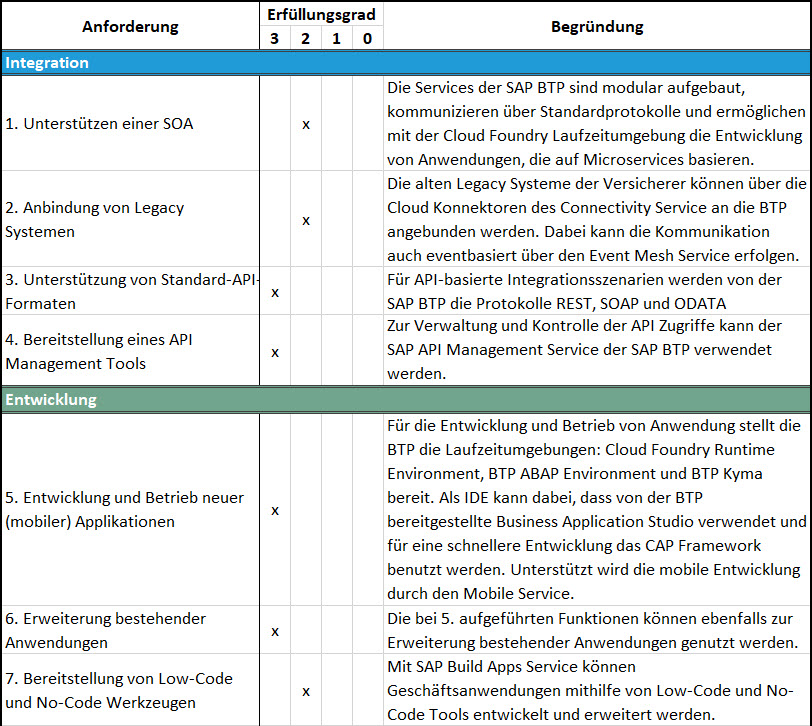
\includegraphics[width=1\textwidth]{img/TTFTeil1E2.jpg}
    %\caption[Vergleich der Task und Technologie Charakteristika Teil 1]{Vergleich der Task und Technologie Charakteristika Teil 1\autocite{TFTeil1}}
    %\footnotetext{eigene Darstellung}
    \label{fig:TTFTeil1}
\end{figure}

\FloatBarrier

\begin{figure}[ht]
    \centering
    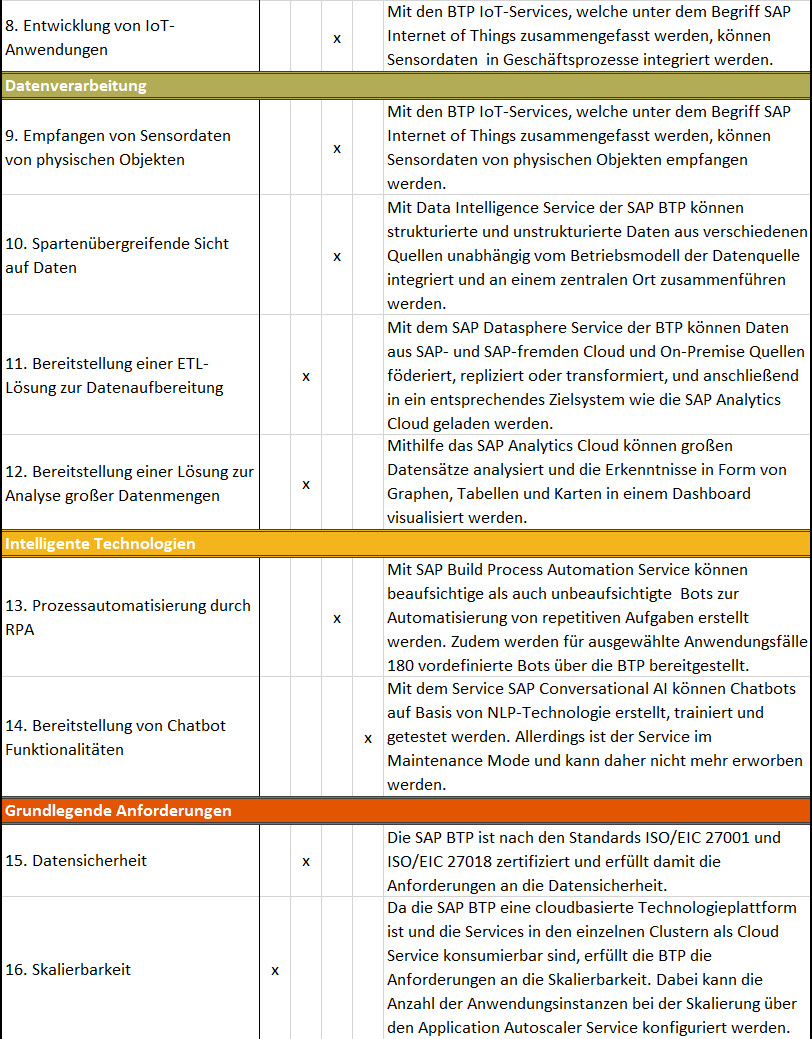
\includegraphics[width=1\textwidth]{img/TTFTeil2E.jpg}
    %\caption[Vergleich der Task und Technologie Charakteristika Teil 2]{Vergleich der Task und Technologie Charakteristika Teil 2\autocite{TFTeil2}}
    %\footnotetext{eigene Darstellung}
    \label{fig:TTFTeil2}
\end{figure}

\FloatBarrier

\begin{figure}[ht]
    \centering
    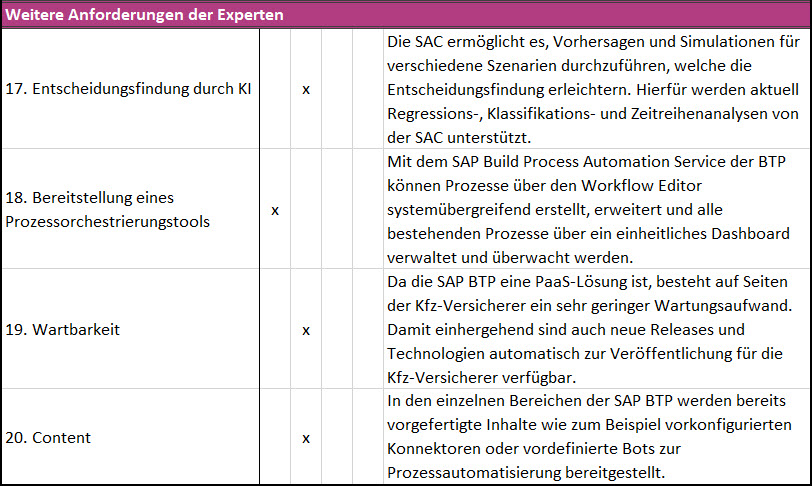
\includegraphics[width=1\textwidth]{img/TTFTeil3E.jpg}
    \caption[Synthese der Task und Technologie Charakteristika ]{Synthese der Task und Technologie Charakteristika \autocite{TTFTeil3}}
    \label{fig:TTFTeil3}
\end{figure}
\footnotetext{eigene Darstellung, Quellen: \cites{GARTNERINC2023}; \cites{GARTNERINC2023b}; \cites{GARTNERINC2023c}; \cites{GARTNERINC2023d}; \cites{GARTNERINC2023e}; \cites{GARTNERINC2023f}; \cites{G22023}; \cites{GARTNERINC2023g} }


%\begin{figure}[ht]
   % \centering
    %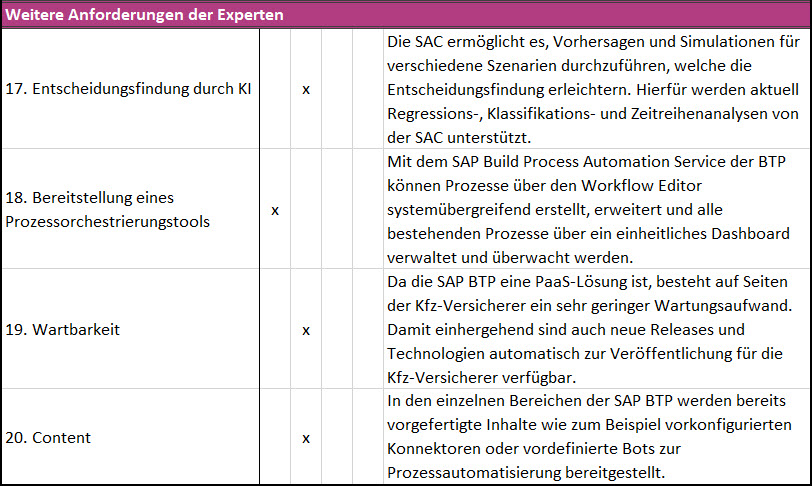
\includegraphics[width=1\textwidth]{img/TTFTeil3E.jpg}
   % \caption[Synthese der Task und Technologie Charakteristika ]{Synthese der Task und Technologie Charakteristika \autocite{TFTeil3}}
   % \footnotetext{eigene Darstellung}
    %\label{fig:TTFTeil3}
%\end{figure}

\FloatBarrier

\improvement{Quellen in die Abbildung der Synthese mit aufnehmen}

\improvement{Worst Case bei Verschiebung der Seiten aufgrund des Textes, punkte 5 und 6 zur 2. Abbildung schieben und ggf. bei Skalierbarkeit die Begründung verkürzen}

Die Synthese der Task- und Technologie-Charakteristika in Abbildung … zeigt, dass bis auf die Anforderung, Chatbot-Funktionalitäten bereitzustellen, die SAP \ac{btp} alle Anforderungen der Kfz-Versicherer an eine digitale Plattform erfüllt. Somit besteht ein sehr hoher Task-Technology-Fit. Weiterhin ist festzustellen, dass die SAP BTP im Vergleich zu konkurrierenden Produkten in den Bereichen Integration, Anwendungsentwicklung und Prozessorchestrierung eine überdurchschnittlich gute Leistung erbringt. Damit hebt sich die SAP BTP in genau den Anforderungsbereichen von den Lösungen der Mitbewerber ab, die für Kfz-Versicherer in den nächsten drei bis fünf Jahren gemäß der Experten besonders wichtig sind (Hier Referenz zur Tabelle mit der Priorisierung der Experten). Folglich ist die SAP BTP als digitale Plattform für Kfz-Versicherer sehr gut geeignet, da sie alle wichtigen Anforderungen durchschnittlich oder überdurchschnittlich erfüllt und die fehlende Funktionalität von den Experten nur mit einer mittleren Wichtigkeit eingestuft wird. 

%Zusätzlich können über die Schnittstellen und Konnektoren auch Services von Drittanbietern, die bspw. Chatbots bereitstellen, an die BTP angebunden werden.

%Folglich können Kfz-Versicherer durch den Einsatz der SAP BTP klare Performanceverbesserungen in ihrer Organisation erzielen und sich damit vom Wettbewerb im Markt differenzieren.



\newpage